As a poor man way to understand the frequency dependence of the charge channel we introduce a "\emph{perpendicular ladder} approximation. This is meant to understand how the ladder type diagrams in the magnetic channel that are always present in all the region of the parameter space affect the frequency dependence in the charge channel, i.e., how ladder diagrams behave in a "perpendicular" ladder resummation.

\begin{itemize}
\item We assume that the magnetic interaction is large and therefore can be computed by RPA, neglecting feedback from other channels. This is an overstimation of the magnetic fluctuations. 

\item From this we compute an effective interaction for the other channels, by approriate frequency and momentum translation ; 

\item Magnetic RPA local effective interaction:

\item \textbf{SCRIVERE FORMULA DELLA BOLLA!}

\begin{equation}
  U_{eff}(\Omega) =\int_{\boldsymbol{Q}} \frac{U}{ 1 - U \Pi^{\Omega}_{\boldsymbol{Q}} }
\end{equation}
(only the momentum integrated interaction enters in the momentum decomposition considered)

\item the charge channel is computed by RPA: 
\begin{equation}
  \Phi_{charge}^{\Omega,\nu,\nu'}(\boldsymbol{Q}) = U_{eff}(\Omega) 
  \left[ 1+  \Pi^{\Omega,\nu}_{\boldsymbol{Q}} U_{eff}(\nu'-\nu) \right]_{\nu,\nu'}^{-1},
\end{equation}
where it is very important to understand the equations as matrix (in the frequency space) equalities. 

\item As one can see in Fig. \ref{Perpladder} the frequency structure obtained for the charge channel reflects the one of fRG (and also of DMF$^2$RG). 
This formula predicts the frequency structure, while certainly giving an overestimate for the effective value of the channel, which has not  to be taken quantitatively. 

\item From figure \ref{bubble} one can understand both the importance of the frequency dependence of the interaction and why the structure is particularly large for the first nonvanishing bosonic frequency. 
Indeed: if the interaction was featureless in the frequency, only the frequency summed bubble would enter in the equations. This, in turn vanishes for $\mathbf{Q}=(0,0)$ and finite frequency.  

\end{itemize}

\begin{figure}
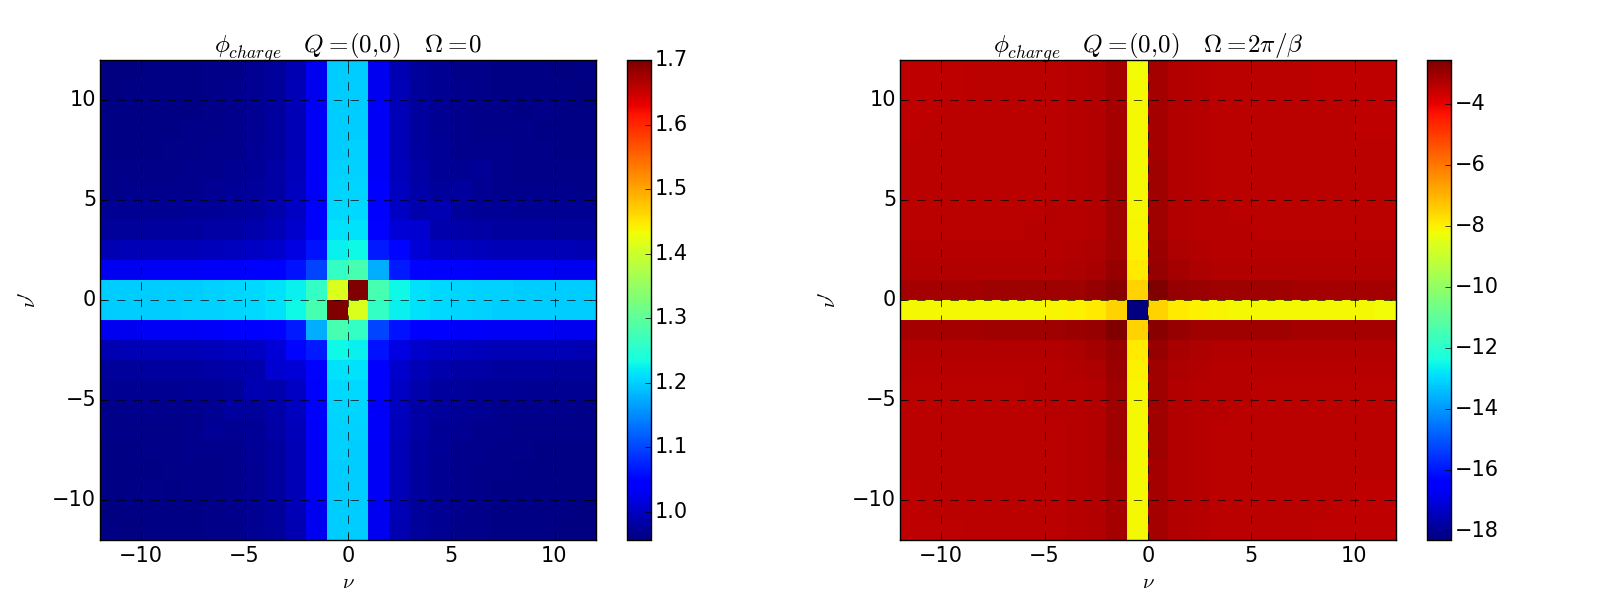
\includegraphics[scale=0.25]{images/Perp_ladder_density.png}
\caption{Charge channel calculated with RPA method for $\Omega=0$ (left) and $\Omega=2\pi/\beta$ (right). }
 \label{Perpladder}
\end{figure}

\begin{figure}
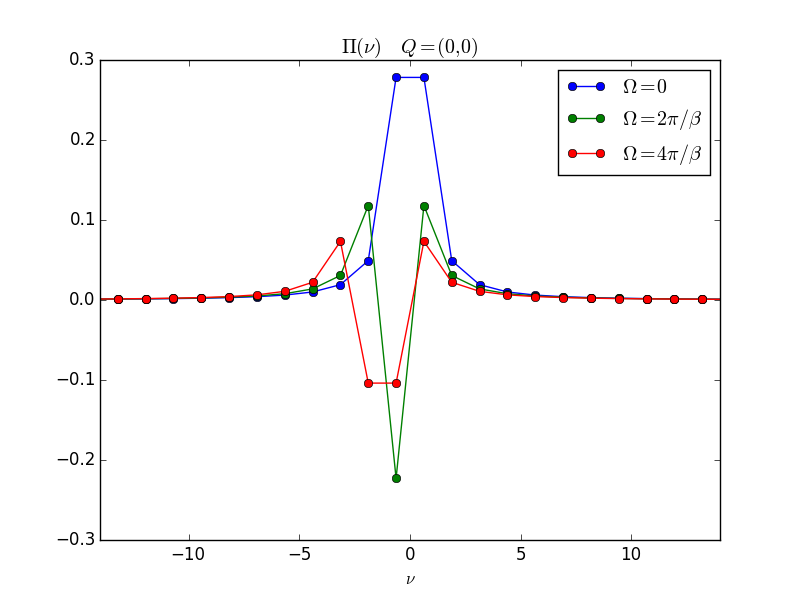
\includegraphics[scale=0.7]{images/Bubble_ph.png}
\caption{PH Bubble as a function of fermionic frequency $\nu$ at $\boldsymbol{Q}=(0,0)$. }
 \label{bubble}
\end{figure}